\documentclass[table,15pt,t]{beamer}

\usepackage{fontspec}
\usepackage{xunicode} %Unicode extras!
\usepackage{xltxtra}  %Fixes
\usepackage{relsize}  %relative font sizing commands
\usepackage{booktabs}
\usepackage{eulervm} %mathfonts
\usepackage{tikz}
\usepackage{listings}
\usepackage{graphicx}
\usepackage{tabularx}
\usepackage{alltt}
\usepackage{ifthen,calc}

\usetheme{Sleek}

\usetikzlibrary{arrows,shapes,shapes.arrows,positioning}
\usetikzlibrary{chains}

\tikzstyle{ds} = [draw, thick, color=oxygenblue, inner sep=0pt, drop shadow]

\setsansfont[Mapping=tex-text]{Trade Gothic LT Std}

\setlength{\fboxsep}{2mm}
\newcommand{\sem}[1]{\ensuremath{[\![#1]\!]}}

\title{Optimized Translation of Clafer Models to Alloy}
\author{Kacper Bak}
\institute{\small Generative Software Development Lab\\University of Waterloo}
\date{CS744 Course Project. July 21, 2011}

\newcommand{\vmiddle}[1]{
  \vspace{\stretch{1}}
  #1
  \vspace{\stretch{1}}
}

\newcommand{\interframe}[1]{
\begin{frame}{}
\vmiddle{\hmiddle{\Huge #1}}
\end{frame}
}

\newcommand{\mlist}[1]{
\vmiddle{
  \begin{list}{}{}
    #1
  \end{list}
  }
}

\newcommand{\hmiddle}[1]{
  \begin{center}#1\end{center}
}

\newcommand{\twocolumns}[4]{
    \begin{columns}
      \begin{column}{#1\textwidth}
        \begin{overlayarea}{#1\textwidth}{\textheight}
          #2
        \end{overlayarea}
      \end{column}
      \begin{column}{#3\textwidth}
        \begin{overlayarea}{#3\textwidth}{\textheight}
          #4
        \end{overlayarea}
      \end{column}
    \end{columns}
}

\newcounter{i}
\newcommand{\ganimate}[3]{
    \setcounter{i}{0}
    \whiledo{\value{i}<#2}{
      \stepcounter{i}
      \only<\the\value{i}>{\includegraphics[#3]{figs/#1\the\value{i}}}
    }
}

\newcommand{\showCode}[3]{
  \only<#1>{\lstinputlisting[firstline=#2,lastline=#3]{code/telematics.cfr}}
}

\makeatletter
\newcommand{\showCodesStart}[3]{
\setcounter{i}{#1}
\@for\arg:=#3\do{
  \showCode{\value{i}}{#2}{\arg}
\stepcounter{i}
}}
\makeatother

\newcommand{\showCodes}[2]{
\showCodesStart{1}{#1}{#2}
}

% To make the legend for icons in class diagrams
\newcommand{\icon}[1]{\textcircled{\texttt{\textbf{\textit{#1}}}}}

\lstdefinelanguage{Clafer}
{morekeywords={abstract, else, in, no, opt, xor, all, enum, lone, not, or, disj, extends, mux, one, some},
sensitive=true,
morecomment=[l][\footnotesize\itshape]{--},
morecomment=[s][\small\itshape]{{-}{-}},
%basicstyle=\footnotesize,
tabsize=4,
columns=fullflexible,
literate={->}{{$\to$ }}1 {^}{{$\mspace{-3mu}\widehat{\quad}\mspace{-3mu}$}}1
 {<}{$<$ }2 {>}{$>$ }2 {>=}{$\geq$ }2 {<=}{$\leq$ }2
 {<:}{{$<\mspace{-3mu}:$}}2 {:>}{{$:\mspace{-3mu}>$}}2
 {<=>}{{$\Leftrightarrow$ }}2
 {=>}{{$\Rightarrow$ }}2 {+}{$+$ }2 {++}{{$+\mspace{-8mu}+$ }}2
 {\~}{{$\mspace{-3mu}\widetilde{\quad}\mspace{-3mu}$}}1
 {!=}{$\neq$ }2 {*}{${}^{\ast}$}1
 {\#}{$\#$}1
 {\~}{$\neg$}1
 {+}{$+$ }1
}

\lstset{basicstyle=\small,language=Clafer,numbers=none}

\begin{document}

\begin{frame}[plain]
  \vmiddle{\titlepage}
\end{frame}

\begin{frame}{Software Intensive}
  \hmiddle{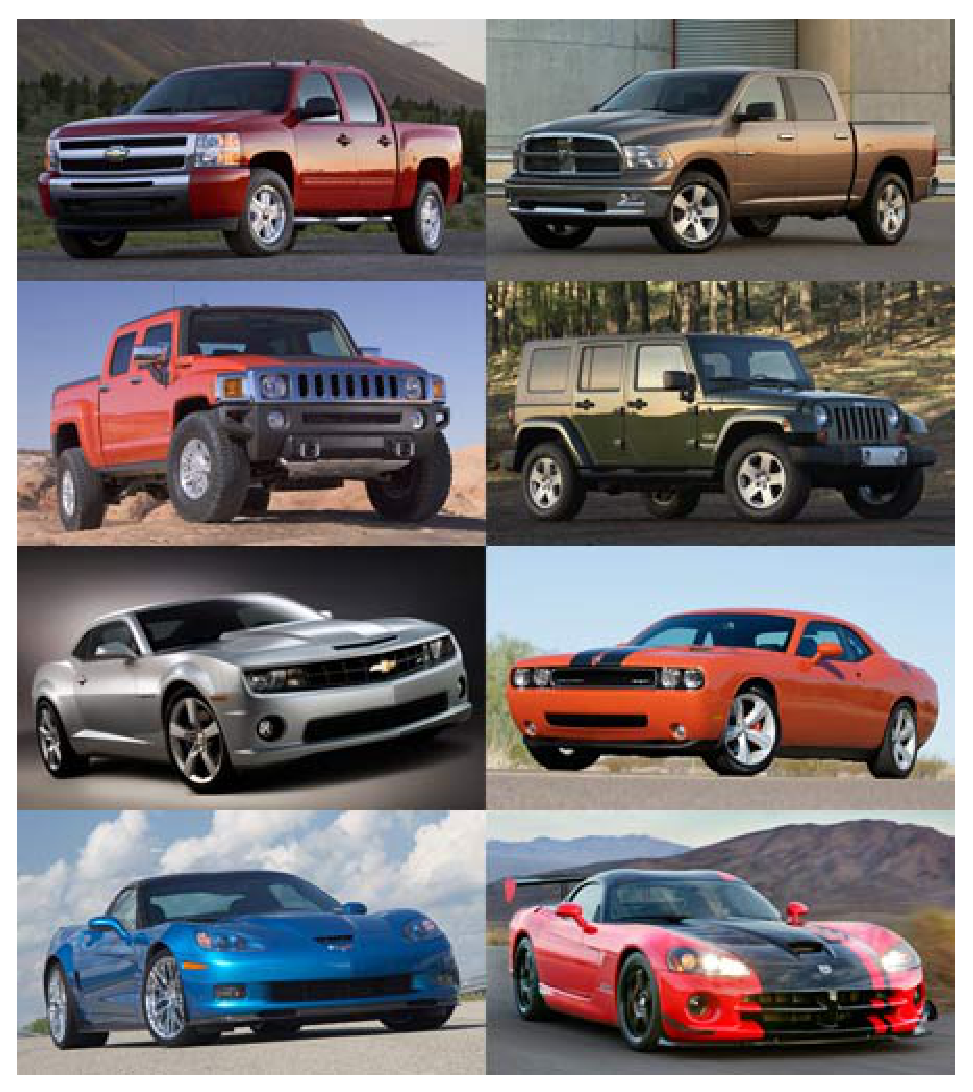
\includegraphics[scale=0.4]{figs/cars}}
\end{frame}

\begin{frame}{Products Come in}
  \hmiddle{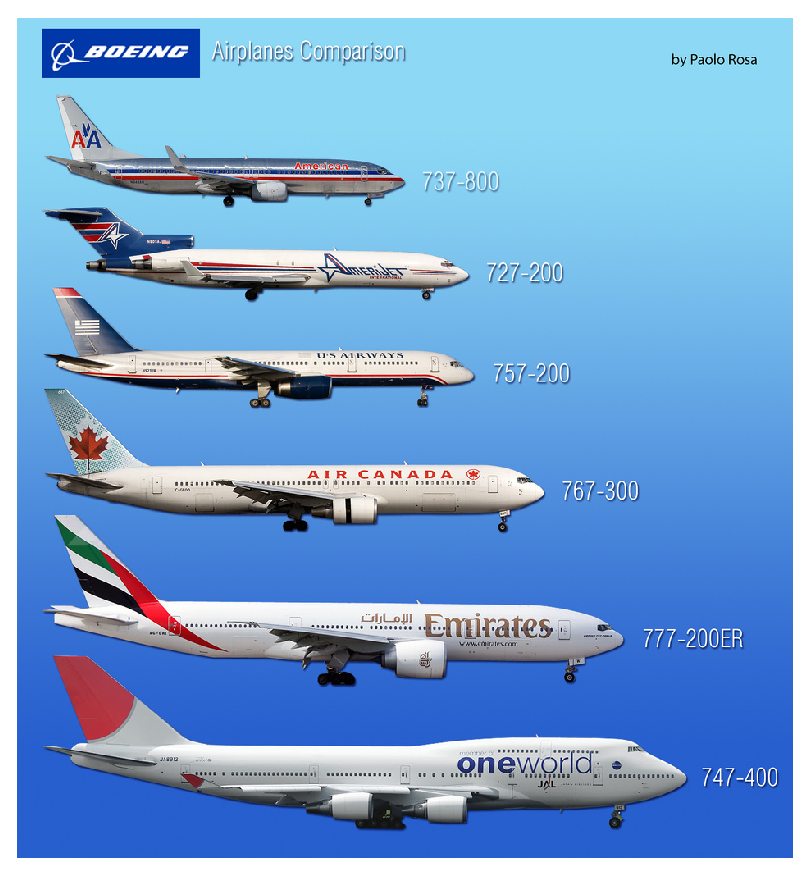
\includegraphics[scale=0.5]{figs/planes}}
\end{frame}

\begin{frame}{Many Variants}
  \hmiddle{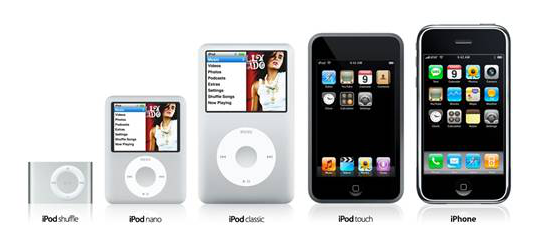
\includegraphics[width=\textwidth]{figs/is}}
\end{frame}

\begin{frame}{Software Product Line}
\newcolumntype{V}{>{\centering\arraybackslash} m{.3\linewidth} }
\begin{tabularx}{\textwidth}{V>{\centering\arraybackslash} m{.18\linewidth}V}
  \begin{tikzpicture}
    \draw (0,0) ellipse (1.2cm and 1.5cm) node {
      \parbox[b]{1cm}{\centering \textbf{Problem\\ Space}}};
  \end{tikzpicture}
  &
  \begin{tikzpicture}
    \node [single arrow, draw] at (0,0) {\textbf{Mapping}};
  \end{tikzpicture}
  &
  \begin{tikzpicture}
    \draw (0,0) ellipse (1.2cm and 1.5cm) node {
      \parbox[b]{1cm}{\centering \textbf{Solution\\ Space}}};
  \end{tikzpicture}\\
  Features & & Assets
\end{tabularx}
\end{frame}

\interframe{Clafer}

\begin{frame}{Clafer}
  \mlist{
    \item Software Product Lines
    \item Textual modeling language
    \item Analyses
  }
\end{frame}

\begin{frame}{SPLs in Clafer}
  \ganimate{all}{6}{width=\textwidth}
\end{frame}

\begin{frame}{The Toolchain}
  \begin{tabularx}{\textwidth}{ccccccccc}
    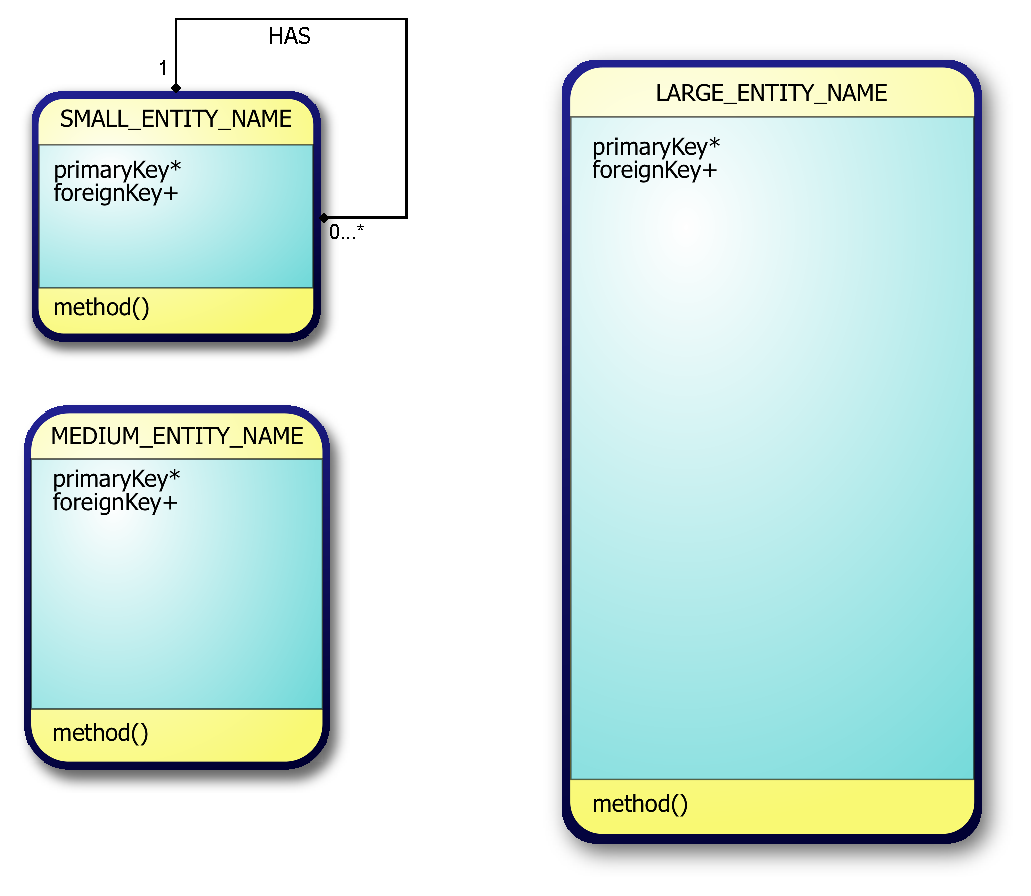
\includegraphics[scale=0.06]{figs/model}
    & $\rightarrow$
    & 
\includegraphics[scale=1]{figs/gears}
    & $\rightarrow$
    & 
\includegraphics[scale=0.3]{figs/document}
    & $\rightarrow$
    & 
\includegraphics[scale=0.7]{figs/alloy}
    & $\rightarrow$
    & $P \land Q$
    \\
    Clafer & & Clafer & & Alloy & & Alloy & & Formula\\
    Model & & Translator & & Model & & Analyzer & &
  \end{tabularx}
\end{frame}

\begin{frame}{Instance Generated by Alloy}
  \hmiddle{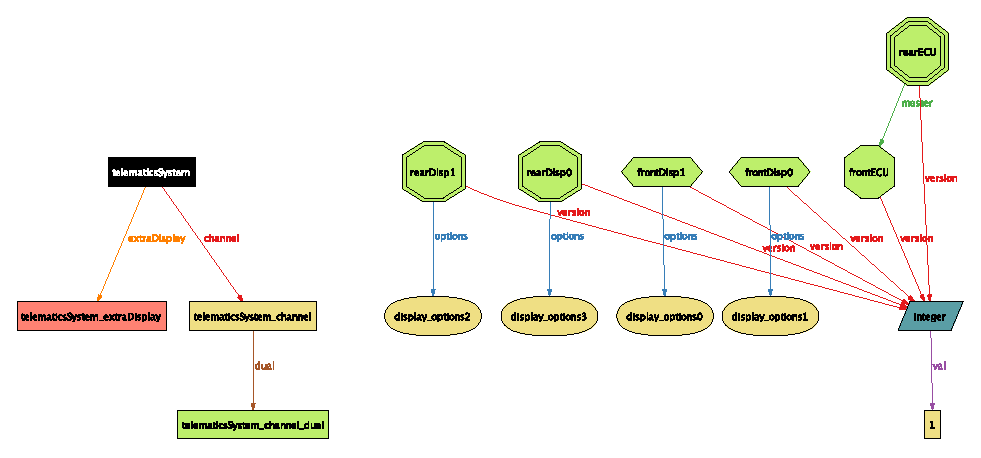
\includegraphics[width=1\textwidth]{figs/tele}}
\end{frame}

\interframe{Problems}

\begin{frame}{Problems}
  \begin{tabularx}{\textwidth}{ccccccccc}
    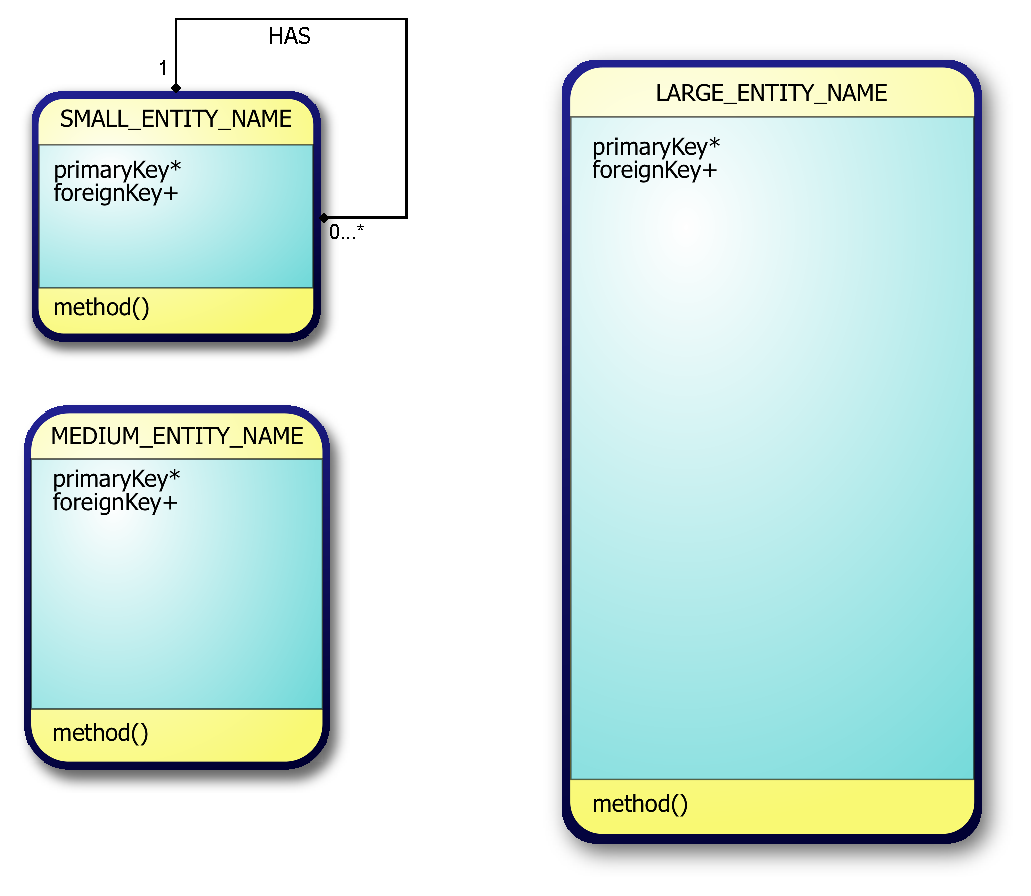
\includegraphics[scale=0.06]{figs/model}
    & $\rightarrow$
    & 
\includegraphics[scale=1]{figs/gears}
    & $\rightarrow$
    & 
\includegraphics[scale=0.3]{figs/document}
    & $\rightarrow$
    & 
\includegraphics[scale=0.7]{figs/alloy}
    & $\rightarrow$
    & $P \land Q$
    \\
    Clafer & & Clafer & & Alloy & & Alloy & & Formula\\
    Model & & Translator & & Model & & Analyzer & &
  \end{tabularx}
  \mlist{
  \item \visible<1->{\textbf{Translation rules heavily influence reasoning time in Alloy}}% bottlenecks
  \item \visible<2->{Large Alloy files (complex models)}
  \item \visible<3->{Ineffective Alloy representation (complex formulas)}
  \item \visible<4->{Slow \textsf{clafer2alloy} translator}
 }
  \begin{tikzpicture}[overlay]
    \draw<2->[red,ultra thick,rounded corners] (5.0,4.0) rectangle (7.0,7.0);
    \draw<3->[red,ultra thick,rounded corners] (10.0,4.0) rectangle (11.75,7.0);
    \draw<4->[red,ultra thick,rounded corners] (2.3,4.0) rectangle (4.3,7.0);
  \end{tikzpicture}
\end{frame}

\interframe{Solution}

\begin{frame}{Solution}
 \mlist{
    \item Refactored and modular code architecture
    \item Intermediate language representation
    \item Optimization of translation rules 
    \item User has control over the translation process
 }
\end{frame}

\begin{frame}{(New) clafer Translator}
\tikzset{>=stealth',every on chain/.append style={join}, every join/.style={->}}
\begin{tikzpicture}[start chain] {
    \node[on chain,rectangle,draw] {Front-end};
    \node[on chain,rectangle,draw] {\parbox[b]{2.5cm}{\centering Intermediate\\ Representation}};
    \node[on chain,rectangle,draw] {Optimizer};
    \node[on chain,rectangle,draw] {\parbox[b]{1.7cm}{\centering Code\\ Generators}};
 }
\end{tikzpicture}

 \mlist{
    \item User can turn on/off modules (has extra knowledge)
    \item Easy to add new code generators
 }
\end{frame}

\interframe{Optimizations}

\begin{frame}{Optimizations}
 \mlist{
    \item Improved name resolution
    \item Dead code removal
    \item Better handling of primitive types (integers)
    \item Better type resolution for references
 }
\end{frame}

\begin{frame}{Simplified Hierarchical Constraints}
  \begin{columns}
    \begin{column}{0.5\textwidth}
      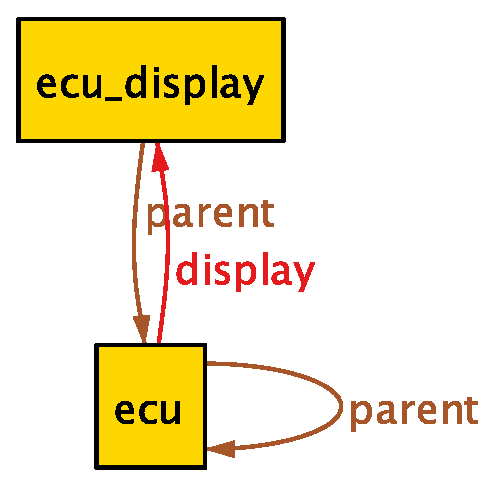
\includegraphics[scale=0.5]{figs/parent-old}
    \end{column}
    \begin{column}{0.5\textwidth}
      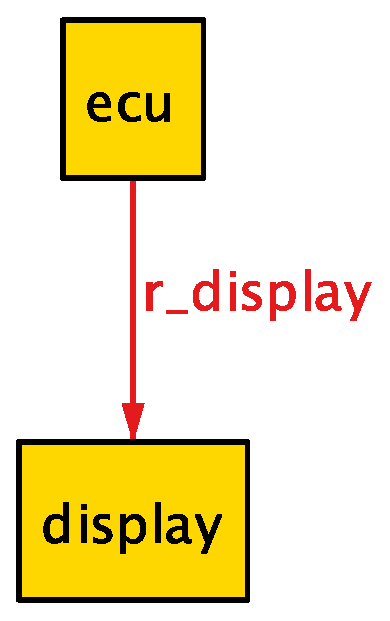
\includegraphics[scale=0.5]{figs/parent-new}
    \end{column}
  \end{columns}
\end{frame}

\begin{frame}[fragile]
  \frametitle{Global Cardinality Constraints}
  \begin{columns}
    \begin{column}{0.5\textwidth}
      \begin{alltt}
        \begin{small}
\textsf{OnBoardComputer} 0..1
  \textsf{Display} 1
        \end{small}
      \end{alltt}
    \end{column}
\pause
    \begin{column}{0.5\textwidth}
      \begin{alltt}
        \begin{small}
\textsf{OnBoardComputer} 0..1
  \textsf{Display} 0..1
        \end{small}
      \end{alltt}
    \end{column}
  \end{columns}

\end{frame}

\begin{frame}[fragile]
  \frametitle{Inheritance Flattening}
  \begin{columns}
    \begin{column}{0.5\textwidth}
      \begin{alltt}
        \begin{small}
\textbf{abstract} \textsf{comp}
  \textsf{version} -> \textsf{integer}

\textsf{display} \textbf{extends} \textsf{comp}
        \end{small}
      \end{alltt}
    \end{column}
\pause
    \begin{column}{0.5\textwidth}
      \begin{alltt}
        \begin{small}
\textsf{display}
  \textsf{version} -> \textsf{integer}
        \end{small}
      \end{alltt}
    \end{column}
  \end{columns}
\end{frame}

\begin{frame}[fragile]
  \frametitle{Model Statistics}
      \begin{alltt}
        \begin{small}
\textsf{ecu} 1..2
  \textsf{display} -> \textsf{integer} 2..3
  \textsf{[display > 2]}
        \end{small}
      \end{alltt}
\pause
      \begin{alltt}
        \begin{small}
All clafers: 2 | Abstract: 0 | Concrete: 1 | References: 1
Constraints: 1
Global scope: 2..6
All names unique: False
        \end{small}
      \end{alltt}
\end{frame}

\begin{frame}{Parameters}
 \mlist{
    \item Dead code removal
    \item Inheritance flattening
    \item Timeout for model translation
    \item Layout resolver options
    \item Checking duplicated names
    \item Name resolver behavior
 }
\end{frame}

\interframe{Evaluation}

\begin{frame}{Input Models}
 \mlist{
    \item Baseline: SLE'10 paper\pause
    \item Feature Models (instantiation)
    \item Meta-Models (instantiation)
    \item FBMTs (liveness, instantiation)\pause
    \item The Linux Kernel
 }
\end{frame}

\begin{frame}{Results}
 \mlist{
    \item Speed: 2-5 times faster
    \item Possible to handle huge models
 }
\end{frame}

\interframe{Conclusion}

\begin{frame}{Conclusion}
 \mlist{
    \item Clafer models can be expressive and analyzable
    \item Alloy Analyzer is slow for big models (even if they are simple)
    \item Possible further optimizations
    \item User knowledge is very useful
 }
\end{frame}

\interframe{Thanks for listening!}

\interframe{Questions?\\[1cm]\normalsize{\textsf{gsd.uwaterloo.ca/clafer}}}

\end{document}
